\renewcommand{\theequation}{\theenumi}
\begin{enumerate}[label=\thesubsection.\arabic*.,ref=\thesubsection.\theenumi]
\numberwithin{equation}{enumi}

\item \solution $p\brak{x, y} = Ax^2 + Bxy + Cy^2 + Dx + Ey + F$ can be represented as follow in the vector form:
\begin{align}
x^T 
\begin{pmatrix}
A & \frac{B}{2} \\
\frac{B}{2} & C
\end{pmatrix}
x + 
\begin{pmatrix}
D & E 
\end{pmatrix}
x + F = 0
\end{align}

\item \begin{flushleft}
The given equation can be represented as follows in the vector form:
\end{flushleft}
\begin{align}
x^T 
\begin{pmatrix}
1 & 0 \\
0 & 0
\end{pmatrix}
x + 
\begin{pmatrix}
-2 & 0 
\end{pmatrix}
x + 0 = 0
\end{align}

\item To find the roots $y=0$:
\begin{align}
x^2 - 2x &= 0 \\
x\brak{x-2} &= 0 \\
x &= 0,2
\end{align}

\item \begin{figure}[!ht]
\centering
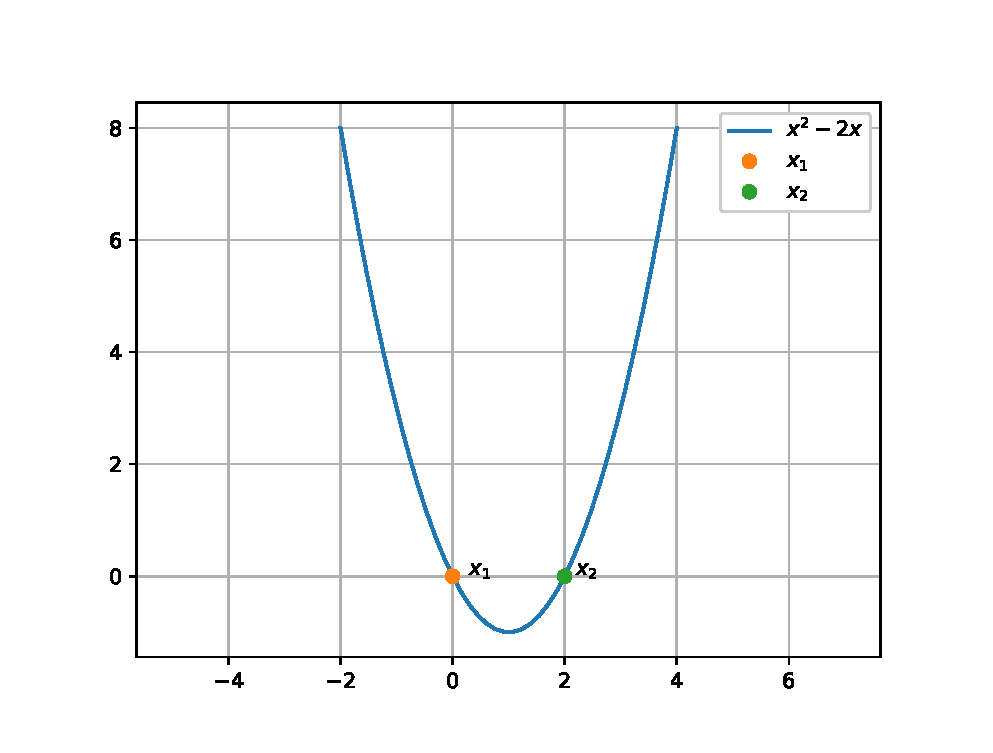
\includegraphics[width=\columnwidth]{./figs/conics_example/quadratic_equation.eps}
\caption{$x^2 -2x$ generated using python}
\label{fig:quadeq_conics_example}
\end{figure} 
The  following Python code generates Fig. \ref{fig:quadeq_conics_example}

\begin{lstlisting}
codes/conics_example/conics.py
\end{lstlisting}
\end{enumerate}